\documentclass[12pt]{book}
\usepackage[margin=.85in]{geometry} % for MARGIN
\usepackage[many]{tcolorbox}    	% for COLORED BOXES (tikz and xcolor included)

\usepackage{multirow}
\usepackage{tabularx}
\usepackage{multicol}   
\usepackage{enumerate}
\usepackage[shortlabels]{enumitem}
\usepackage{varwidth}
\usepackage{tasks}
\usepackage[export]{adjustbox}
\usepackage{array} % For m{} column type

\usepackage{titleps}
\usepackage{setspace}               % for LINE SPACING
\usepackage[⟨options⟩]{fancyhdr}
\usepackage{enumitem}
\setlist{nosep}
\usepackage{tikz}
\usepackage{pgfplots}
\pgfplotsset{compat=1.5.1}
\usetikzlibrary{datavisualization}
\usetikzlibrary{datavisualization.formats.functions}

\newcommand{\D}{\displaystyle}
\newcommand\Mydiv[2]{%
$\strut#1$\kern.25em\smash{\raise.3ex\hbox{$\big)$}}\mkern-8mu
        \overline{\enspace\strut#2}}


\setlength\parindent{0pt}   % killing indentation for all the text
\setstretch{1.3}            % setting line spacing to 1.3
\setlength\columnsep{0.25in} % setting length of column separator
\pagestyle{fancy}           % setting pagestyle to be headings

\usepackage[]{titlesec}

\fancyhead[L]{Math V04 - College Algebra}
\fancyhead[R]{Christina Papazacharioudakis}

\tcbset{
    sharp corners,
    colback = white,
    before skip = 0.2cm,    % add extra space before the box
    after skip = 0.5cm      % add extra space after the box
}                           % setting global options for tcolorbox

    \newtcolorbox{boxR}{
    fontupper = \color{black}, % font color
    boxrule = 1.5pt,
    colframe = black,
    rounded corners,
    arc = 5pt   % corners roundness
}



\begin{document}


{\Large \textbf{5.4 Dividing Polynomials}}
\vspace{1mm}

{\large \textbf{Using Long Division to Divide Polynomials}}
\vspace{1mm}

Just as we can use long division to divide numbers, we can employ a similar process to divide polynomials.  Before we get started on polynomial division, let's review long division for numbers first.

\vspace{5mm}

For example, lets divide $178$ by $3$ using long division. We call $178$ the \underline{\hspace{30mm}} (the number being divided), and $3$ the  \underline{\hspace{30mm}} (the number dividing the dividend).

\vspace{5mm}
A way we can represent this division is: $178 \div 3$ or $\D \frac{178}{3}$. For long division, we write: 
\vspace{110mm}

Another way to look at this solution is as a sum of parts: 
\begin{align*}
\text{dividend } &= \text{(divisor}\cdot \text{quotient) } + \text{ remainder} \\
&=   
\end{align*}


\vspace{15mm}

Now let's apply this process to polynomials...

\newpage 

Each term of the polynomial that we are dividing become the placeholders that we saw for real numbers. We also focus on the highest power of our divisor when dividing. 
\vspace{5mm}

For example, we will use long division for $\D (2x^3-3x^2+4x+5) \div (x+2)$. 

\vspace{150mm}

We can also make sense of this long division as a sum of parts as we did previously: 
\vspace{20mm}

\centerline{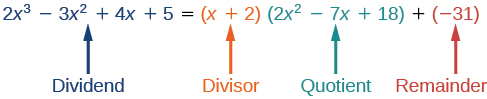
\includegraphics[scale=1.2]{Chapter 5/5.4-figure1.jpeg}}

\newpage

\begin{boxR}
    \textbf{The Division Algorithm}
    \hspace{1mm}
    \hline
    \hspace{2mm}
    
    The \textbf{Division Algorithm} states that, given a polynomial dividend $f(x)$ and a non-zero polynomial divisor $d(x)$ where the degree of $d(x)$  is less than or equal to the degree of $f(x)$, there exist unique polynomials $q(x)$ and  $r(x)$ where 
    $$ f(x) = d(x)q(x) + r(x)$$
    The quotient is $q(x)$ and the remainder is $r(x)$.
    \vspace{1mm}
    
    If $r(x)=0$, then $f(x)=d(x)q(x)$. That is, the divisor is one of the factors of $f(x)$!
\end{boxR}
\bigskip


\underline{\textbf{Example 1 - Use Long Division to Divide a Second-Degree Polynomial}}

Divide $5x^2+3x-2$ by $x+1$.
\vspace{120mm}

Notice that because we got a remainder of zero, $\left[r(x)=0\right]$, applying long division in this situation gave us the factored form of a polynomial! In the future, we will be using long division to help us find all the factors of a polynomial.
\newpage

\underline{\textbf{Example 2 - Use Long Division to Divide a Third-Degree Polynomial}}

Divide $6x^3+11x^2-31x+15$ by $3x-2$.


\newpage
{\large \textbf{Using Synthetic Division to Divide Polynomials}}
\vspace{2mm}

Polynomial long division can be a lot to manage because we are keeping track of all the different terms in the computation, and repeating these involved steps until we get a remainder. We now go over a more efficient and less awkward way to divide polynomials.
\vspace{2mm}

\textbf{Synthetic Division} is a short hand method for dividing polynomials when the divisor is a linear factor with a leading coefficient of one. In other words, the divisor is of the form $(x+a)$ where $a$ is a constant.  Let's illustrate this with an example. 
\vspace{2mm}

Let's divide $3x^3-2x^2+x-4$ by $x+3$ using long division first:

\newpage

\begin{boxR}
    \textbf{How To}
    \vspace{1mm}
    \hline
    \vspace{2mm}
    \textbf{Use synthetic division for polynomials with a divisor of the form $(x+a)$.}
    \begin{enumerate}
        \item Write $-a$ for the divisor.
        \item Write the coefficients of the dividend horizontally. Add zeros for any missing terms. 
        \item Bring the leading coefficient down. 
        \item Multiply the leading coefficient by $-a$. Write the product in the next column.
        \item Add the terms in the second column. 
        \item Multiply the result by $-a$. Write the product in the next column. 
        \item Repeat steps 5 and 6 for remaining columns. 
        \item Use the bottom numbers to write the quotient. The number in the last column is the remainder. 
    \end{enumerate}
\end{boxR}
\bigskip 

\underline{\textbf{Example 3 - Use Synthetic Division to Divide a Third-Degree Polynomial}}

Use synthetic division to divide $4x^3+10x^2-6x-20$ by $x+2$.

\newpage

\underline{\textbf{Example 4 - Use Synthetic Division to Divide a Fourth-Degree Polynomial}}

Use synthetic division to divide $-9x^3+10x^3+7x^2-6$ by $x-1$.






\end{document}


